\subsubsection{Viguetas piso tipo}
    \begin{itemize}
        \item \textbf{Vigueta 1}\\
            \begin{figure}[H]
                \centering
                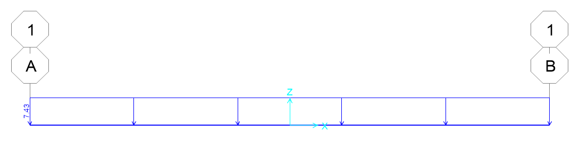
\includegraphics[width=0.9\linewidth]{images/viguetas/VT1 EP.png}
                \caption{Diagrama de carga (1.2D+1.6L) para la vigueta VT1 de entrepiso}
                \label{fig:W VT1 EP}
            \end{figure}
            
            \begin{figure}[H]
                \centering
                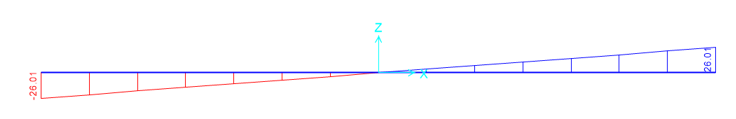
\includegraphics[width=0.9\linewidth]{images/viguetas/CORT VT1 EP.png}
                \caption{Diagrama de Cortante para la vigueta VT1 de entrepiso}
                \label{fig:v VT1 EP}
            \end{figure}
            
             \begin{figure}[H]
                \centering
                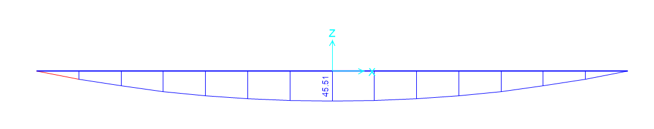
\includegraphics[width=0.9\linewidth]{images/viguetas/MOM VT1 EP.png}
                \caption{Diagrama de momento para la vigueta VT1 de entrepiso}
                \label{fig:M VT1 EP}
            \end{figure}
            
            \item \textbf{Vigueta 2}\\
            \begin{figure}[H]
                \centering
                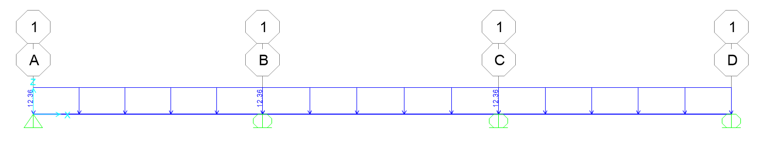
\includegraphics[width=0.9\linewidth]{images/viguetas/VT2 EP.png}
                \caption{Diagrama de carga (1.2D+1.6L) para la vigueta VT2 de entrepiso}
                \label{fig:W VT2 EP}
            \end{figure}
            
            \begin{figure}[H]
                \centering
                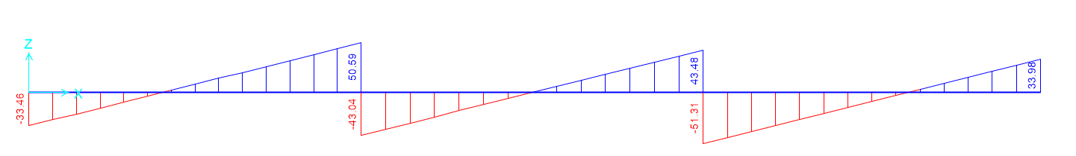
\includegraphics[width=0.9\linewidth]{images/viguetas/CORT VT2 EP.png} 
                \caption{Diagrama de Cortante para la vigueta VT2 de entrepiso}
                \label{fig:v VT2 EP}
            \end{figure}
            
             \begin{figure}[H]
                \centering
                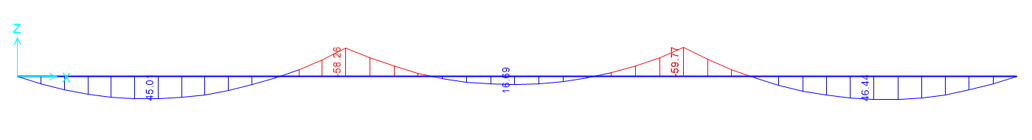
\includegraphics[width=0.9\linewidth]{images/viguetas/MOM VT2 EP.png} 
                \caption{Diagrama de momento para la vigueta VT2 de entrepiso}
                \label{fig:M VT2 EP}
            \end{figure}
            
             \item \textbf{Vigueta 3}\\
            \begin{figure}[H]
                \centering
                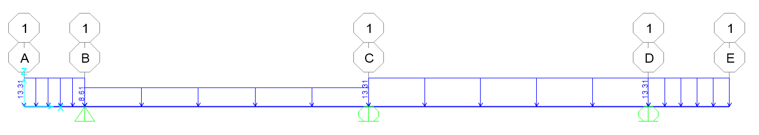
\includegraphics[width=0.9\linewidth]{images/viguetas/VT3 EP.png} 
                \caption{Diagrama de carga (1.2D+1.6L) para la vigueta VT3 de entrepiso}
                \label{fig:W VT3 EP}
            \end{figure}
            
            \begin{figure}[H]
                \centering
                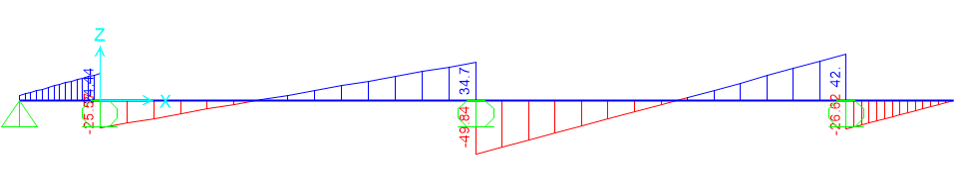
\includegraphics[width=0.9\linewidth]{images/viguetas/CORT VT3 EP.png} 
                \caption{Diagrama de Cortante para la vigueta VT3 de entrepiso}
                \label{fig:v VT3 EP}
            \end{figure}
            
             \begin{figure}[H]
                \centering
                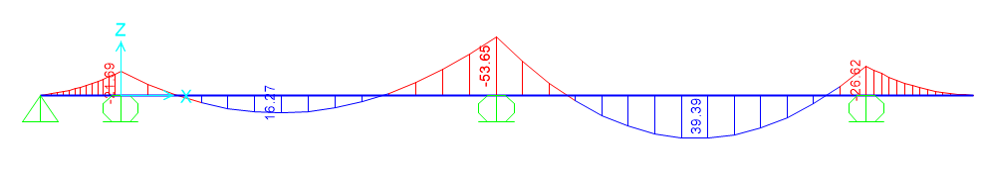
\includegraphics[width=0.9\linewidth]{images/viguetas/MOM VT3 EP.png} 
                \caption{Diagrama de momento para la vigueta VT3 de entrepiso}
                \label{fig:M VT3 EP}
            \end{figure}
            
            \item \textbf{Vigueta 4}\\
            \begin{figure}[H]
                \centering
                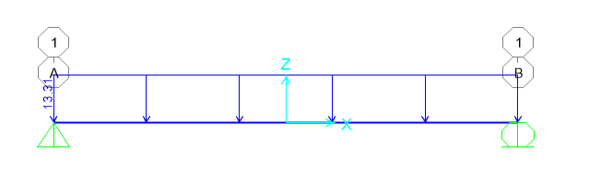
\includegraphics[width=0.9\linewidth]{images/viguetas/VT4 EP.png}
                \caption{Diagrama de carga (1.2D+1.6L) para la vigueta VT4 de entrepiso}
                \label{fig:W VT4 EP}
            \end{figure}
            
            \begin{figure}[H]
                \centering
                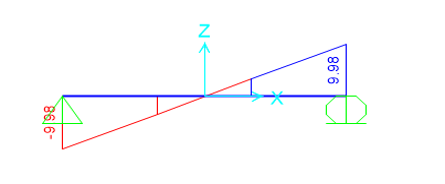
\includegraphics[width=0.9\linewidth]{images/viguetas/CORT VT4 EP.png} 
                \caption{Diagrama de Cortante para la vigueta VT4 de entrepiso}
                \label{fig:v VT4 EP}
            \end{figure}
            
             \begin{figure}[H]
                \centering
                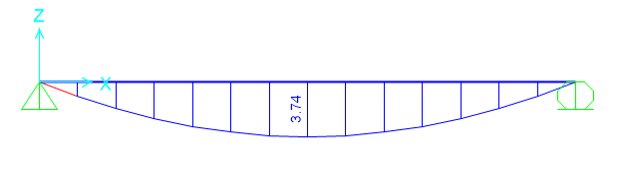
\includegraphics[width=0.9\linewidth]{images/viguetas/MOM VT4 EP.png} 
                \caption{Diagrama de momento para la vigueta VT4 de entrepiso}
                \label{fig:M VT4 EP}
            \end{figure}
            
            
            \item \textbf{Vigueta 5}\\
            \begin{figure}[H]
                \centering
                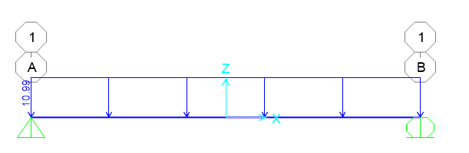
\includegraphics[width=0.9\linewidth]{images/viguetas/VT5 EP.png} 
                \caption{Diagrama de carga (1.2D+1.6L) para la vigueta VT5 de entrepiso}
                \label{fig:W VT5 EP}
            \end{figure}
            
            \begin{figure}[H]
                \centering
                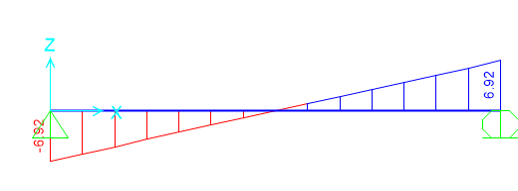
\includegraphics[width=0.9\linewidth]{images/viguetas/CORT VT5 EP.png} 
                \caption{Diagrama de Cortante para la vigueta VT5 de entrepiso}
                \label{fig:v VT5 EP}
            \end{figure}
            
             \begin{figure}[H]
                \centering
                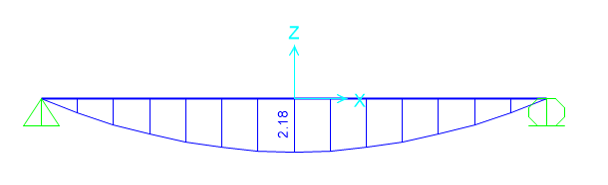
\includegraphics[width=0.9\linewidth]{images/viguetas/MOM VT5 EP.png} 
                \caption{Diagrama de momento para la vigueta VT5 de entrepiso}
                \label{fig:M VT5 EP}
            \end{figure}
            
            \item \textbf{Vigueta 6}\\
            \begin{figure}[H]
                \centering
                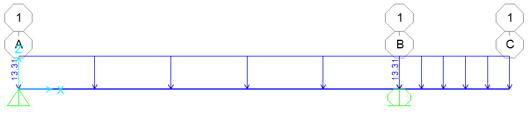
\includegraphics[width=0.9\linewidth]{images/viguetas/VT6 EP.png} 
                \caption{Diagrama de carga (1.2D+1.6L) para la vigueta VT6 de entrepiso}
                \label{fig:W VT6 EP}
            \end{figure}
            
            \begin{figure}[H]
                \centering
                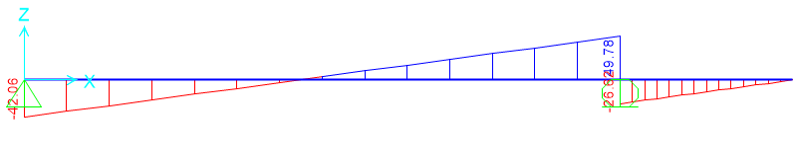
\includegraphics[width=0.9\linewidth]{images/viguetas/CORT VT6 EP.png} 
                \caption{Diagrama de Cortante para la vigueta VT6 de entrepiso}
                \label{fig:v VT6 EP}
            \end{figure}
            
             \begin{figure}[H]
                \centering
                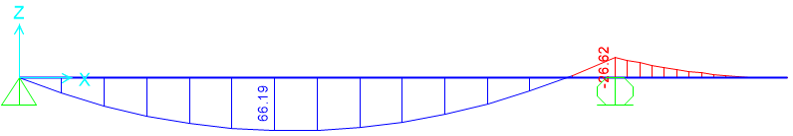
\includegraphics[width=0.9\linewidth]{images/viguetas/MOM VT6 EP.png} 
                \caption{Diagrama de momento para la vigueta VT6 de entrepiso}
                \label{fig:M VT6 EP}
            \end{figure}
            
            \item \textbf{Vigueta 7}\\
            \begin{figure}[H]
                \centering
                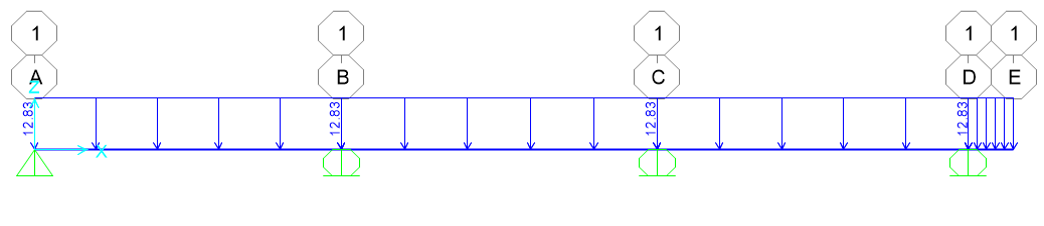
\includegraphics[width=0.9\linewidth]{images/viguetas/VT7 EP.png} 
                \caption{Diagrama de carga (1.2D+1.6L) para la vigueta VT7 de entrepiso}
                \label{fig:W VT7 EP}
            \end{figure}
            
            \begin{figure}[H]
                \centering
                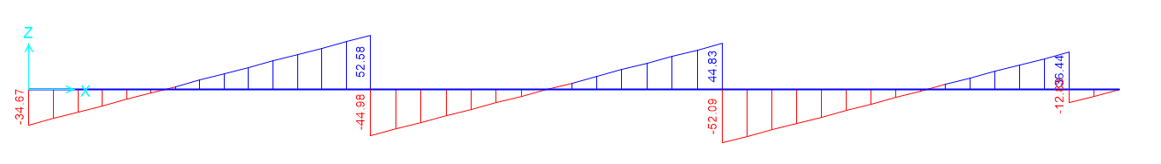
\includegraphics[width=0.9\linewidth]{images/viguetas/CORT VT7 EP.png}
                \caption{Diagrama de Cortante para la vigueta VT7 de entrepiso}
                \label{fig:v VT7 EP}
            \end{figure}
            
             \begin{figure}[H]
                \centering
                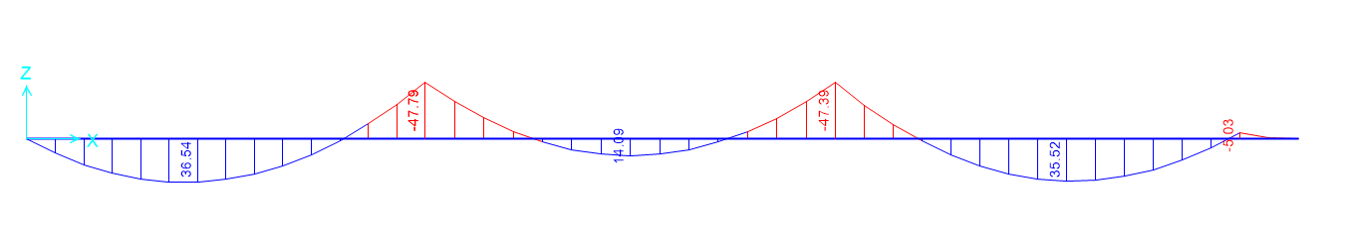
\includegraphics[width=0.9\linewidth]{images/viguetas/MOM VT7 CUB.png} 
                \caption{Diagrama de momento para la vigueta VT7 de entrepiso}
                \label{fig:M VT7 EP}
            \end{figure}
\end{itemize}

\subsubsection{Viguetas cubierta}

\begin{itemize}
    \item \textbf{Vigueta 1}\\
    \begin{figure}[H]
                \centering
                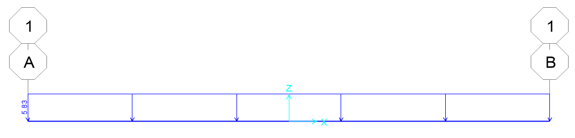
\includegraphics[width=0.9\linewidth]{images/viguetas/VT1 CUB.png} 
                \caption{Diagrama de carga (1.2D+1.6L) para la vigueta VT1 de cubierta}
                \label{fig:W VT1 CUB}
            \end{figure}
            
            \begin{figure}[H]
                \centering
                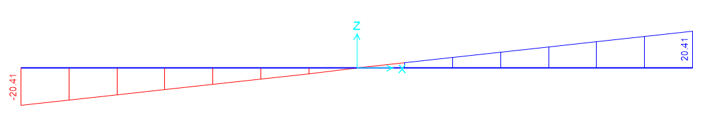
\includegraphics[width=0.9\linewidth]{images/viguetas/CORT VT1 CUB.png}
                \caption{Diagrama de Cortante para la vigueta VT1 de cubierta}
                \label{fig:v VT7 CUB}
            \end{figure}
            
             \begin{figure}[H]
                \centering
                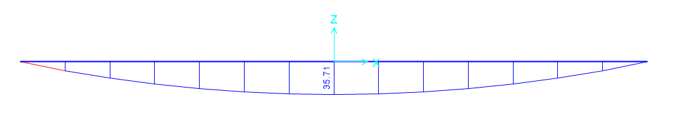
\includegraphics[width=0.9\linewidth]{images/viguetas/MOM VT1 CUB.png} 
                \caption{Diagrama de momento para la vigueta VT1 de cubierta}
                \label{fig:M VT1 CUB}
            \end{figure}
        
        \item \textbf{Vigueta 2}\\
        \begin{figure}[H]
                \centering
                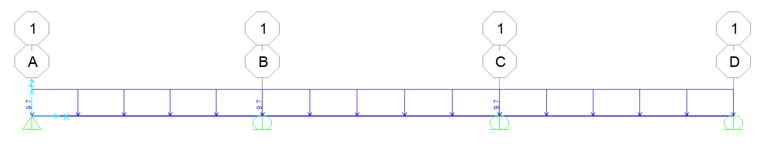
\includegraphics[width=0.9\linewidth]{images/viguetas/VT2 CUB.png} 
                \caption{Diagrama de carga (1.2D+1.6L) para la vigueta VT2 de cubierta}
                \label{fig:W VT2 CUB}
            \end{figure}
            
            \begin{figure}[H]
                \centering
                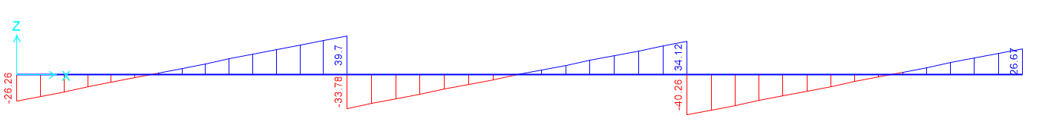
\includegraphics[width=0.9\linewidth]{images/viguetas/CORT VT2 CUB.png}
                \caption{Diagrama de Cortante para la vigueta VT2 de cubierta}
                \label{fig:v VT2 CUB}
            \end{figure}
            
             \begin{figure}[H]
                \centering
                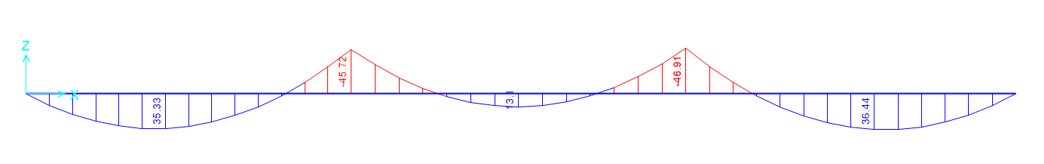
\includegraphics[width=0.9\linewidth]{images/viguetas/MOM VT2 CUB.png} 
                \caption{Diagrama de momento para la vigueta VT2 de cubierta}
                \label{fig:M VT2 CUB}
            \end{figure}
            
            \item \textbf{Vigueta 7'}\\
        \begin{figure}[H]
                \centering
                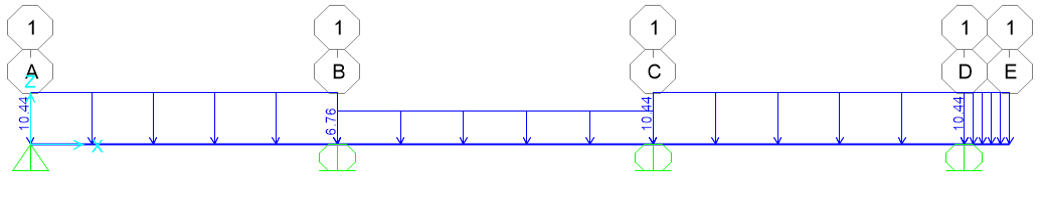
\includegraphics[width=0.9\linewidth]{images/viguetas/VT7 CUB'.png} 
                \caption{Diagrama de carga (1.2D+1.6L) para la vigueta VT7' de cubierta}
                \label{fig:W VT7' CUB}
            \end{figure}
            
            \begin{figure}[H]
                \centering
                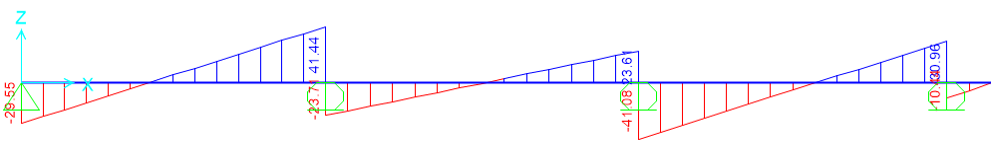
\includegraphics[width=0.9\linewidth]{images/viguetas/CORT VT 7 CUB'.png}
                \caption{Diagrama de Cortante para la vigueta VT7' de cubierta}
                \label{fig:v VT7' CUB}
            \end{figure}
            
             \begin{figure}[H]
                \centering
                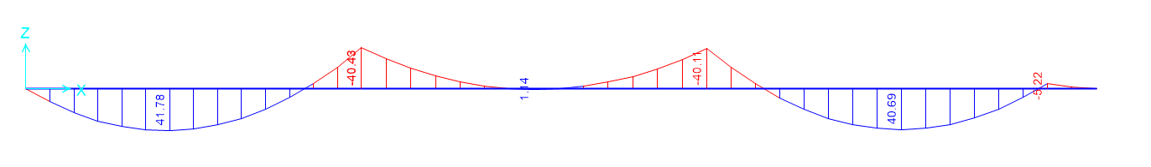
\includegraphics[width=0.9\linewidth]{images/viguetas/MOM VT7 CUB'.png} 
                \caption{Diagrama de momento para la vigueta VT7' de cubierta}
                \label{fig:M VT7' CUB}
            \end{figure}
            
            
               \item \textbf{Vigueta 7}\\
        \begin{figure}[H]
                \centering
                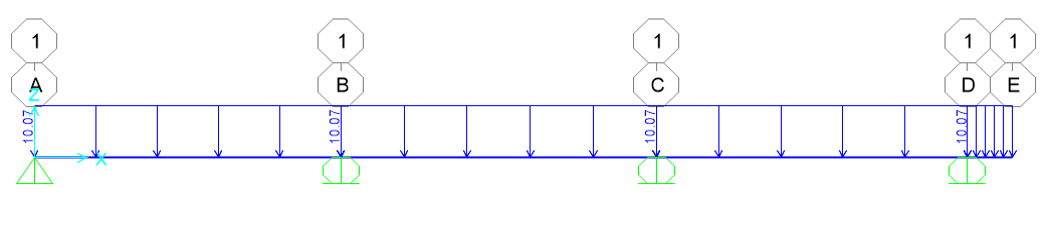
\includegraphics[width=0.9\linewidth]{images/viguetas/VT7 CUB.png} 
                \caption{Diagrama de carga (1.2D+1.6L) para la vigueta VT7 de cubierta}
                \label{fig:W VT7 CUB}
            \end{figure}
            
            \begin{figure}[H]
                \centering
                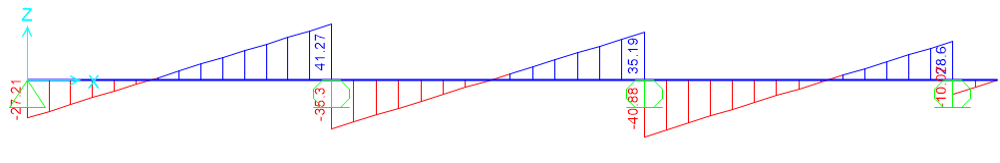
\includegraphics[width=0.9\linewidth]{images/viguetas/CORT VT 7 CUB.png}
                \caption{Diagrama de Cortante para la vigueta VT7 de cubierta}
                \label{fig:v VT7 CUB}
            \end{figure}
            
             \begin{figure}[H]
                \centering
                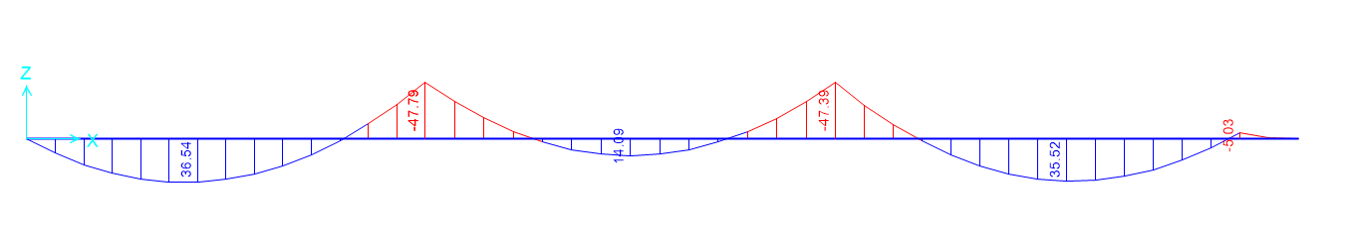
\includegraphics[width=0.9\linewidth]{images/viguetas/MOM VT7 CUB.png} 
                \caption{Diagrama de momento para la vigueta VT7 de cubierta}
                \label{fig:M VT7 CUB}
            \end{figure}
            
              \item \textbf{Vigueta 8}\\
        \begin{figure}[H]
                \centering
                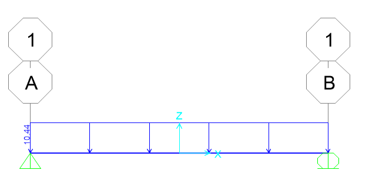
\includegraphics[width=0.9\linewidth]{images/viguetas/VT8 CUB.png} 
                \caption{Diagrama de carga (1.2D+1.6L) para la vigueta VT8 de cubierta}
                \label{fig:W VT8 CUB}
            \end{figure}
            
            \begin{figure}[H]
                \centering
                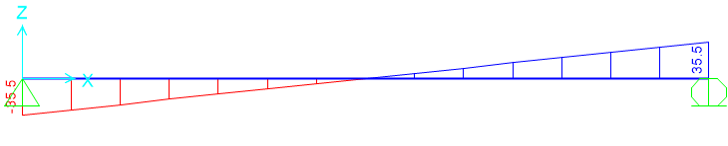
\includegraphics[width=0.9\linewidth]{images/viguetas/CORT VT8 CUB.png}
                \caption{Diagrama de Cortante para la vigueta VT8 de cubierta}
                \label{fig:v VT8 CUB}
            \end{figure}
            
             \begin{figure}[H]
                \centering
                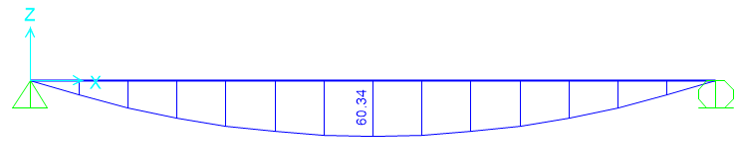
\includegraphics[width=0.9\linewidth]{images/viguetas/MOM VT8 CUB.png} 
                \caption{Diagrama de momento para la vigueta VT8 de cubierta}
                \label{fig:M VT8 CUB}
            \end{figure}
            
            
             \item \textbf{Vigueta 9}\\
        \begin{figure}[H]
                \centering
                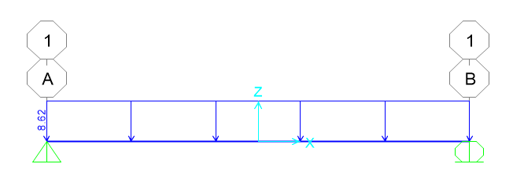
\includegraphics[width=0.9\linewidth]{images/viguetas/VT9 CUB.png} 
                \caption{Diagrama de carga (1.2D+1.6L) para la vigueta VT9 de cubierta}
                \label{fig:W VT9 CUB}
            \end{figure}
            
            \begin{figure}[H]
                \centering
                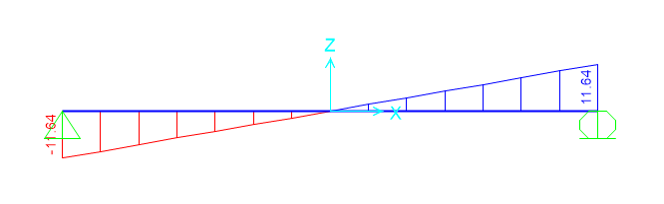
\includegraphics[width=0.9\linewidth]{images/viguetas/CORT V9 CUB.png}
                \caption{Diagrama de Cortante para la vigueta VT9 de cubierta}
                \label{fig:v VT9 CUB}
            \end{figure}
            
             \begin{figure}[H]
                \centering
                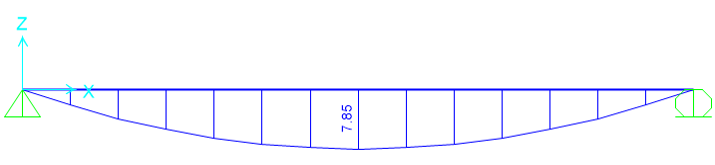
\includegraphics[width=0.9\linewidth]{images/viguetas/MOM VT9 CUB.png} 
                \caption{Diagrama de momento para la vigueta VT9 de cubierta}
                \label{fig:M VT9 CUB}
            \end{figure}
            
             \item \textbf{Vigueta 10}\\
        \begin{figure}[H]
                \centering
                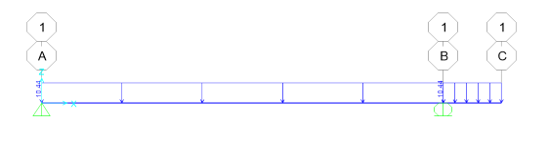
\includegraphics[width=0.9\linewidth]{images/viguetas/VT10 CUB.png} 
                \caption{Diagrama de carga (1.2D+1.6L) para la vigueta VT10 de cubierta}
                \label{fig:W VT10 CUB}
            \end{figure}
            
            \begin{figure}[H]
                \centering
                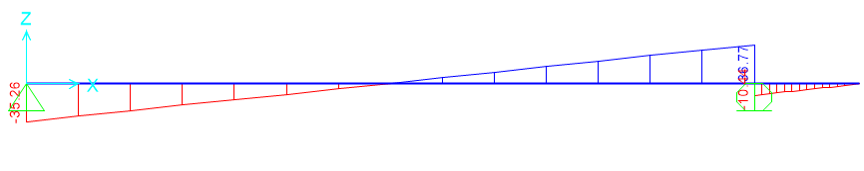
\includegraphics[width=0.9\linewidth]{images/viguetas/CORT VT10 CUB.png}
                \caption{Diagrama de Cortante para la vigueta VT10 de cubierta}
                \label{fig:v VT10 CUB}
            \end{figure}
            
             \begin{figure}[H]
                \centering
                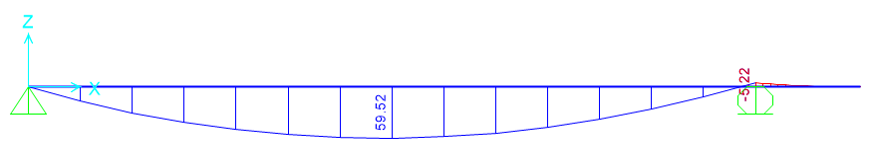
\includegraphics[width=0.9\linewidth]{images/viguetas/MOM VT10 CUB.png} 
                \caption{Diagrama de momento para la vigueta VT10 de cubierta}
                \label{fig:M VT10 CUB}
            \end{figure}
    
\end{itemize}